
\section{A Little Configuration}

\subsection{Letting m2e know your password}

\begin{enumerate}
\item Click \textbf{Edit} (or \textbf{Window} depending on your OS) $\rightarrow$ \textbf{Preferences}, and choose \textbf{Maven} $\rightarrow$ \textbf{User Settings}, and find the default Maven setting path for your system. See Figure \ref{eclipse-03-maven-setting}.

\item Create the \verb|settings.xml| file at the given directory, and copy the text in Listing \ref{settings} into the file, which will store your ID and passwords. Remember to replace \verb|ID| and \verb|PASSWORD| with your personal Maven project repository account we provide you, and also don't upload this file to any remote repository or share it with others.

\item Go back to \textbf{Edit} (or \textbf{Window}) $\rightarrow$ \textbf{Preferences}, and choose \textbf{Maven} $\rightarrow$ \textbf{User Settings} again, you will see the plugin could find the setting file you specified (see Figure \ref{eclipse-04-maven-setting-back}).
% and click \textbf{Update settings}. You will be able to see the repository is now being refreshed. 

\begin{figure}[t]
\hspace{-3em}
\begin{minipage}{0.5\textwidth}
\centering
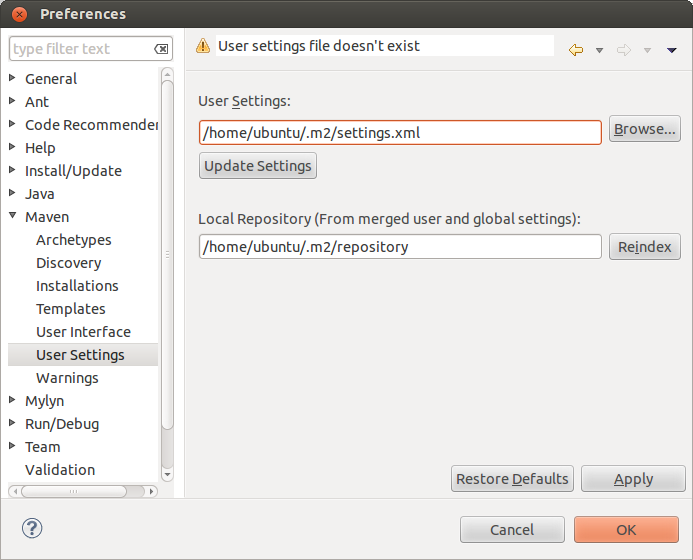
\includegraphics[scale=0.3]{eclipse-03-maven-setting}
\caption{Eclipse maven user profile setting\label{eclipse-03-maven-setting}}
\end{minipage}
\hfill
\begin{minipage}{0.5\textwidth}
\centering
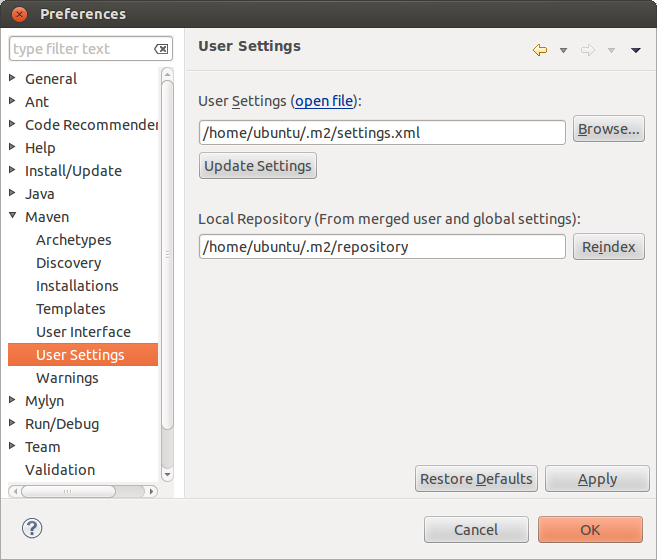
\includegraphics[scale=0.3]{eclipse-04-maven-setting-back}
\caption{Eclipse maven user profile setting\label{eclipse-04-maven-setting-back}}
\end{minipage}
\hspace{-3em}
\end{figure}

\lstinputlisting[language=XML,float,linewidth=1.1\textwidth,caption=Configuring settings.xml,label=settings]{settings.xml}

\end{enumerate}

\subsection{Importing Apache UIMA code style template}

To development a software as a team, members should always adopt the same code conventions to improve the readability and maintainability of the project. We suggest you to view the \emph{Code Conventions for the Java Programming Language} at \url{http://www.oracle.com/technetwork/java/codeconv-138413.html}, which was published from Oracle. For our course homeworks, you are required to adopt a set of more specific coding conventions from Apache UIMA project. Details can be found at \url{http://uima.apache.org/codeConventions.html}. At the bottom of the page, you could find a link to download the Eclipse code style template\footnote{\url{http://uima.apache.org/downloads/ApacheUima_EclipseCodeStylePrefs.xml}}.

\begin{enumerate}
\item Download the template and save it in your local filesystem.
\item Click \textbf{Window} $\rightarrow$ \textbf{Preferences}, then go to \textbf{Java} $\rightarrow$ \textbf{Code Style} $\rightarrow$ \textbf{Formatter}, and click \textbf{Import\ldots}. 
\end{enumerate}

Remember before you finish editing a Java file, press \textbf{Ctrl+Shift+F} to perform an automatic code formation.

Another optional but useful tool for you to check your code style is the Eclipse Checkstyle plug-in. You can learn how to download and install the plug-in at \url{http://eclipse-cs.sourceforge.net/}.
